% Options for packages loaded elsewhere
% Options for packages loaded elsewhere
\PassOptionsToPackage{unicode}{hyperref}
\PassOptionsToPackage{hyphens}{url}
\PassOptionsToPackage{dvipsnames,svgnames,x11names}{xcolor}
%
\documentclass[
  letterpaper,
  DIV=11,
  numbers=noendperiod]{scrreprt}
\usepackage{xcolor}
\usepackage{amsmath,amssymb}
\setcounter{secnumdepth}{5}
\usepackage{iftex}
\ifPDFTeX
  \usepackage[T1]{fontenc}
  \usepackage[utf8]{inputenc}
  \usepackage{textcomp} % provide euro and other symbols
\else % if luatex or xetex
  \usepackage{unicode-math} % this also loads fontspec
  \defaultfontfeatures{Scale=MatchLowercase}
  \defaultfontfeatures[\rmfamily]{Ligatures=TeX,Scale=1}
\fi
\usepackage{lmodern}
\ifPDFTeX\else
  % xetex/luatex font selection
\fi
% Use upquote if available, for straight quotes in verbatim environments
\IfFileExists{upquote.sty}{\usepackage{upquote}}{}
\IfFileExists{microtype.sty}{% use microtype if available
  \usepackage[]{microtype}
  \UseMicrotypeSet[protrusion]{basicmath} % disable protrusion for tt fonts
}{}
\makeatletter
\@ifundefined{KOMAClassName}{% if non-KOMA class
  \IfFileExists{parskip.sty}{%
    \usepackage{parskip}
  }{% else
    \setlength{\parindent}{0pt}
    \setlength{\parskip}{6pt plus 2pt minus 1pt}}
}{% if KOMA class
  \KOMAoptions{parskip=half}}
\makeatother
% Make \paragraph and \subparagraph free-standing
\makeatletter
\ifx\paragraph\undefined\else
  \let\oldparagraph\paragraph
  \renewcommand{\paragraph}{
    \@ifstar
      \xxxParagraphStar
      \xxxParagraphNoStar
  }
  \newcommand{\xxxParagraphStar}[1]{\oldparagraph*{#1}\mbox{}}
  \newcommand{\xxxParagraphNoStar}[1]{\oldparagraph{#1}\mbox{}}
\fi
\ifx\subparagraph\undefined\else
  \let\oldsubparagraph\subparagraph
  \renewcommand{\subparagraph}{
    \@ifstar
      \xxxSubParagraphStar
      \xxxSubParagraphNoStar
  }
  \newcommand{\xxxSubParagraphStar}[1]{\oldsubparagraph*{#1}\mbox{}}
  \newcommand{\xxxSubParagraphNoStar}[1]{\oldsubparagraph{#1}\mbox{}}
\fi
\makeatother


\usepackage{longtable,booktabs,array}
\usepackage{calc} % for calculating minipage widths
% Correct order of tables after \paragraph or \subparagraph
\usepackage{etoolbox}
\makeatletter
\patchcmd\longtable{\par}{\if@noskipsec\mbox{}\fi\par}{}{}
\makeatother
% Allow footnotes in longtable head/foot
\IfFileExists{footnotehyper.sty}{\usepackage{footnotehyper}}{\usepackage{footnote}}
\makesavenoteenv{longtable}
\usepackage{graphicx}
\makeatletter
\newsavebox\pandoc@box
\newcommand*\pandocbounded[1]{% scales image to fit in text height/width
  \sbox\pandoc@box{#1}%
  \Gscale@div\@tempa{\textheight}{\dimexpr\ht\pandoc@box+\dp\pandoc@box\relax}%
  \Gscale@div\@tempb{\linewidth}{\wd\pandoc@box}%
  \ifdim\@tempb\p@<\@tempa\p@\let\@tempa\@tempb\fi% select the smaller of both
  \ifdim\@tempa\p@<\p@\scalebox{\@tempa}{\usebox\pandoc@box}%
  \else\usebox{\pandoc@box}%
  \fi%
}
% Set default figure placement to htbp
\def\fps@figure{htbp}
\makeatother





\setlength{\emergencystretch}{3em} % prevent overfull lines

\providecommand{\tightlist}{%
  \setlength{\itemsep}{0pt}\setlength{\parskip}{0pt}}



 


% === cover-style.tex ===
\usepackage{fontspec}
\usepackage{xcolor}
\usepackage{pagecolor}

% -------------------------------------------------------
% CONFIGURACIÓN DE FUENTES
% -------------------------------------------------------
% ⚠️ Asegúrate de colocar tus fuentes en esta carpeta sin tildes ni espacios:
% /Users/eliseo/Documents/fonts/
%
% Contenido esperado:
%   - RobotoVariable.ttf
%   - RobotoVariable-Italic.ttf

\setmainfont[
  Path = /Users/eliseo/Documents/fonts/,
  UprightFont = {RobotoVariable.ttf},
  ItalicFont  = {RobotoVariable-Italic.ttf}
]{Roboto}

% Variantes de peso para usar dentro del documento
\newfontfamily\robotoLight[
  Path = /Users/eliseo/Documents/fonts/,
  UprightFont = {RobotoVariable.ttf},
  FontFace = {l}{n}{+wght=300}
]{Roboto Light}

\newfontfamily\robotoMedium[
  Path = /Users/eliseo/Documents/fonts/,
  UprightFont = {RobotoVariable.ttf},
  FontFace = {m}{n}{+wght=500}
]{Roboto Medium}

\newfontfamily\robotoRegular[
  Path = /Users/eliseo/Documents/fonts/,
  UprightFont = {RobotoVariable.ttf},
  FontFace = {r}{n}{+wght=400}
]{Roboto Regular}

% -------------------------------------------------------
% COLORES PERSONALIZADOS
% -------------------------------------------------------
\definecolor{coverblue}{HTML}{0F3754}  % azul oscuro corporativo
\definecolor{coverwhite}{HTML}{FFFFFF} % blanco puro

% -------------------------------------------------------
% ESTILO GLOBAL DEL DOCUMENTO
% -------------------------------------------------------
\AtBeginDocument{%
  % Forzamos Roboto como fuente sans-serif predeterminada
  \renewcommand{\familydefault}{\sfdefault}
  \setmainfont[
    Path = /Users/eliseo/Documents/fonts/,
    UprightFont = {RobotoVariable.ttf},
    ItalicFont  = {RobotoVariable-Italic.ttf}
  ]{Roboto}
  \robotoRegular
}
\KOMAoption{captions}{tableheading}
\makeatletter
\@ifpackageloaded{bookmark}{}{\usepackage{bookmark}}
\makeatother
\makeatletter
\@ifpackageloaded{caption}{}{\usepackage{caption}}
\AtBeginDocument{%
\ifdefined\contentsname
  \renewcommand*\contentsname{Table of contents}
\else
  \newcommand\contentsname{Table of contents}
\fi
\ifdefined\listfigurename
  \renewcommand*\listfigurename{List of Figures}
\else
  \newcommand\listfigurename{List of Figures}
\fi
\ifdefined\listtablename
  \renewcommand*\listtablename{List of Tables}
\else
  \newcommand\listtablename{List of Tables}
\fi
\ifdefined\figurename
  \renewcommand*\figurename{Figure}
\else
  \newcommand\figurename{Figure}
\fi
\ifdefined\tablename
  \renewcommand*\tablename{Table}
\else
  \newcommand\tablename{Table}
\fi
}
\@ifpackageloaded{float}{}{\usepackage{float}}
\floatstyle{ruled}
\@ifundefined{c@chapter}{\newfloat{codelisting}{h}{lop}}{\newfloat{codelisting}{h}{lop}[chapter]}
\floatname{codelisting}{Listing}
\newcommand*\listoflistings{\listof{codelisting}{List of Listings}}
\makeatother
\makeatletter
\makeatother
\makeatletter
\@ifpackageloaded{caption}{}{\usepackage{caption}}
\@ifpackageloaded{subcaption}{}{\usepackage{subcaption}}
\makeatother
\usepackage{bookmark}
\IfFileExists{xurl.sty}{\usepackage{xurl}}{} % add URL line breaks if available
\urlstyle{same}
\hypersetup{
  pdftitle={Libro de Consultas},
  pdfauthor={Unidad de Análisis y Estudios},
  colorlinks=true,
  linkcolor={blue},
  filecolor={Maroon},
  citecolor={Blue},
  urlcolor={Blue},
  pdfcreator={LaTeX via pandoc}}


\title{Libro de Consultas}
\usepackage{etoolbox}
\makeatletter
\providecommand{\subtitle}[1]{% add subtitle to \maketitle
  \apptocmd{\@title}{\par {\large #1 \par}}{}{}
}
\makeatother
\subtitle{Tendencias electorales (varias encuestas)}
\author{Unidad de Análisis y Estudios}
\date{}
\begin{document}
\maketitle

\thispagestyle{empty}
\pagenumbering{gobble}
\pagecolor{coverblue}
\color{coverwhite}

\vspace*{\fill}
\begin{center}
{\robotoMedium\fontsize{36}{42}\selectfont Libro de Consultas}\\[1.5em]
{\robotoRegular\fontsize{22}{28}\selectfont Tendencias electorales (varias encuestas)}\\[2em]
{\robotoLight\fontsize{18}{24}\selectfont Eliseo}\\[2em]
\today
\end{center}
\vspace*{\fill}

\pagecolor{white}
\pagenumbering{arabic}
\clearpage

\renewcommand*\contentsname{Table of contents}
{
\hypersetup{linkcolor=}
\setcounter{tocdepth}{2}
\tableofcontents
}

\bookmarksetup{startatroot}

\chapter{Libro de Consultas}\label{libro-de-consultas}

Tendencias electorales (varias encuestas)

\hfill\break

\thispagestyle{empty}
\pagenumbering{gobble}
\pagecolor{coverblue}
\color{coverwhite}

\vspace*{\fill}
\begin{center}
{\robotoMedium\fontsize{36}{42}\selectfont Libro de Consultas}\\[1.5em]
{\robotoRegular\fontsize{22}{28}\selectfont Tendencias electorales (varias encuestas)}\\[2em]
{\robotoLight\fontsize{18}{24}\selectfont Eliseo}\\[2em]
\today
\end{center}
\vspace*{\fill}

\pagecolor{white}
\pagenumbering{arabic}
\clearpage

\bookmarksetup{startatroot}

\chapter{Introducción}\label{introducciuxf3n}

Este documento recoge la intención de voto a los principales partidos y
otras variables relacionadas, basadas en datos acumulados de encuestas
desde septiembre de 2023.\\
A continuación se muestran los resultados desagregados por sexo, edad y
otras variables de interés.

\part{1 · Intención de voto (IDV)}

\chapter{Intención de voto (IDV)}\label{intenciuxf3n-de-voto-idv-1}

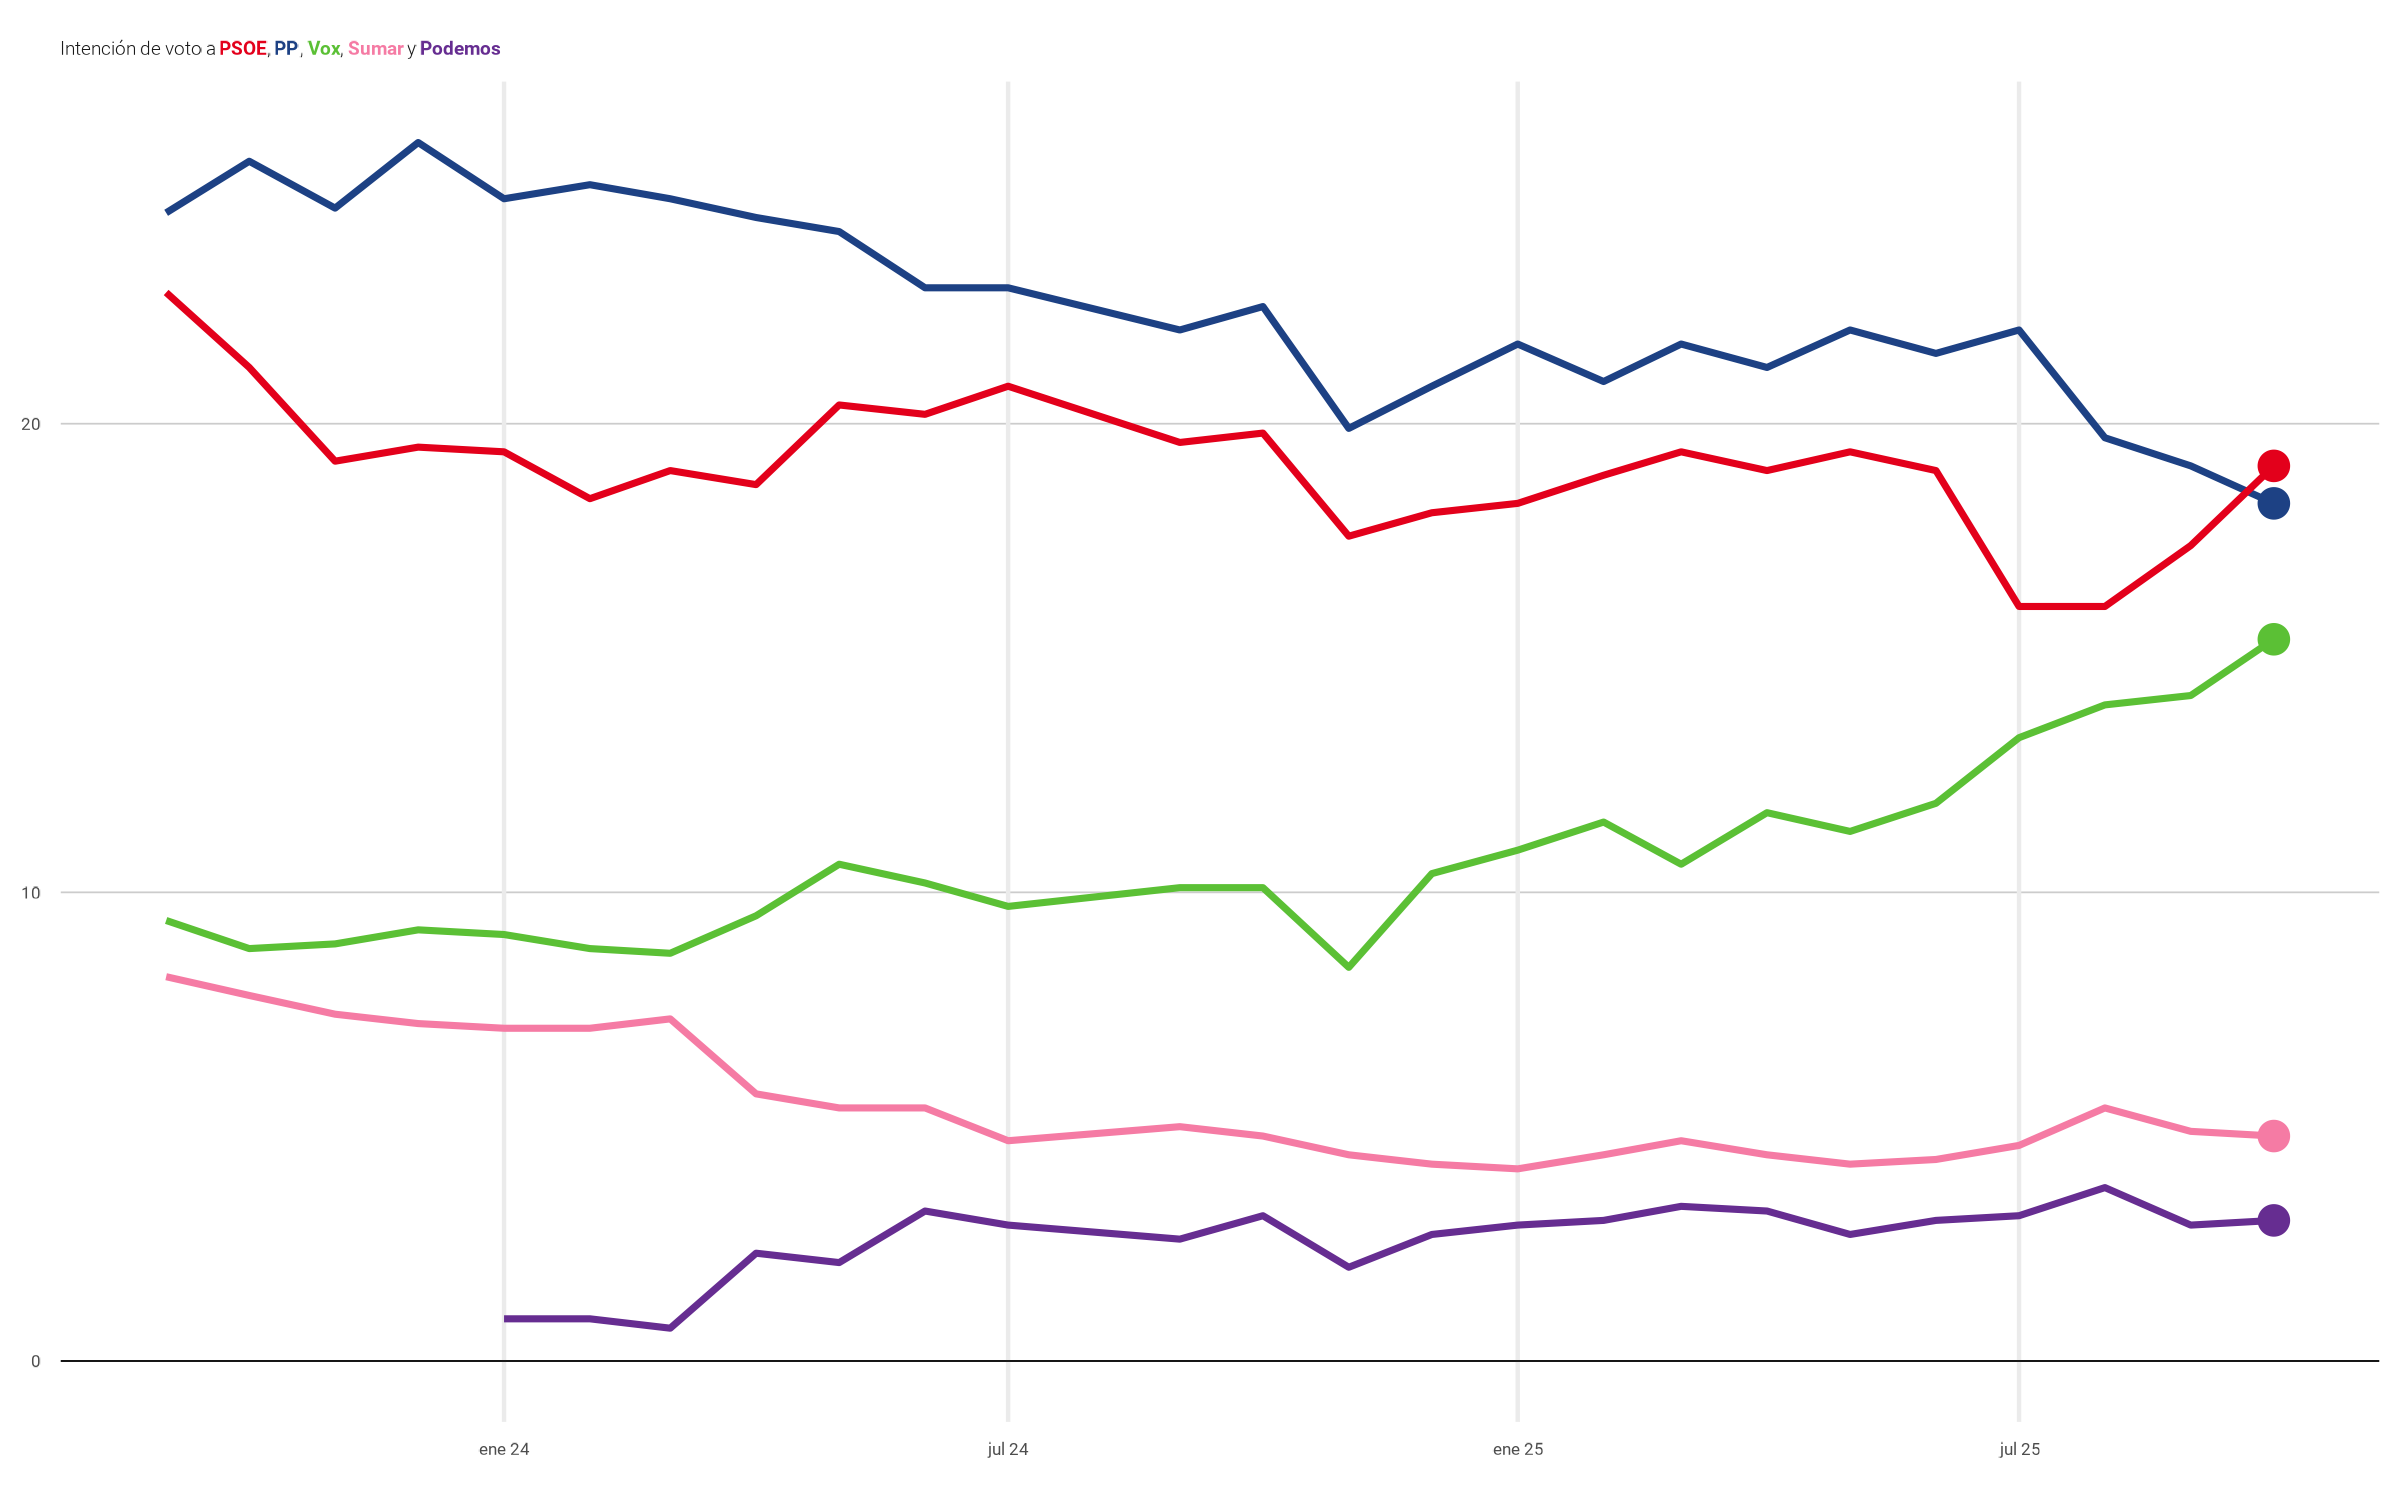
\includegraphics[width=8in,height=\textheight,keepaspectratio]{figures/p_idv_static.png}

{PP}: En septiembre de 2023 un 24.6\% afirmaba que les votaría, hoy lo
hace un 18.3\%, una diferencia de -6.3 puntos. El dato más bajo fue
18.3\% en octubre de 2025, y el más alto 26.5\% en diciembre de 2023.

{PSOE}: En septiembre de 2023 un 24.1\% afirmaba que les votaría, hoy lo
hace un 19.1\%, una diferencia de -5 puntos. El dato más bajo fue 16\%
en julio de 2025, y el más alto 24.1\% en septiembre de 2023.

{Podemos}: En enero de 2024 un 0.8\% afirmaba que les votaría, hoy lo
hace un 3\%, una diferencia de 2.2 puntos. El dato más bajo fue 0.6\% en
marzo de 2024, y el más alto 3.7\% en agosto de 2025.

{Sumar}: En septiembre de 2023 un 9.2\% afirmaba que les votaría, hoy lo
hace un 4.8\%, una diferencia de -4.4 puntos. El dato más bajo fue 4\%
en enero de 2025, y el más alto 9.2\% en septiembre de 2023.

{Vox}: En septiembre de 2023 un 9.1\% afirmaba que les votaría, hoy lo
hace un 15.4\%, una diferencia de 6.3 puntos. El dato más bajo fue 8.4\%
en noviembre de 2024, y el más alto 15.4\% en octubre de 2025.

\chapter{Intención de voto por
género}\label{intenciuxf3n-de-voto-por-guxe9nero}

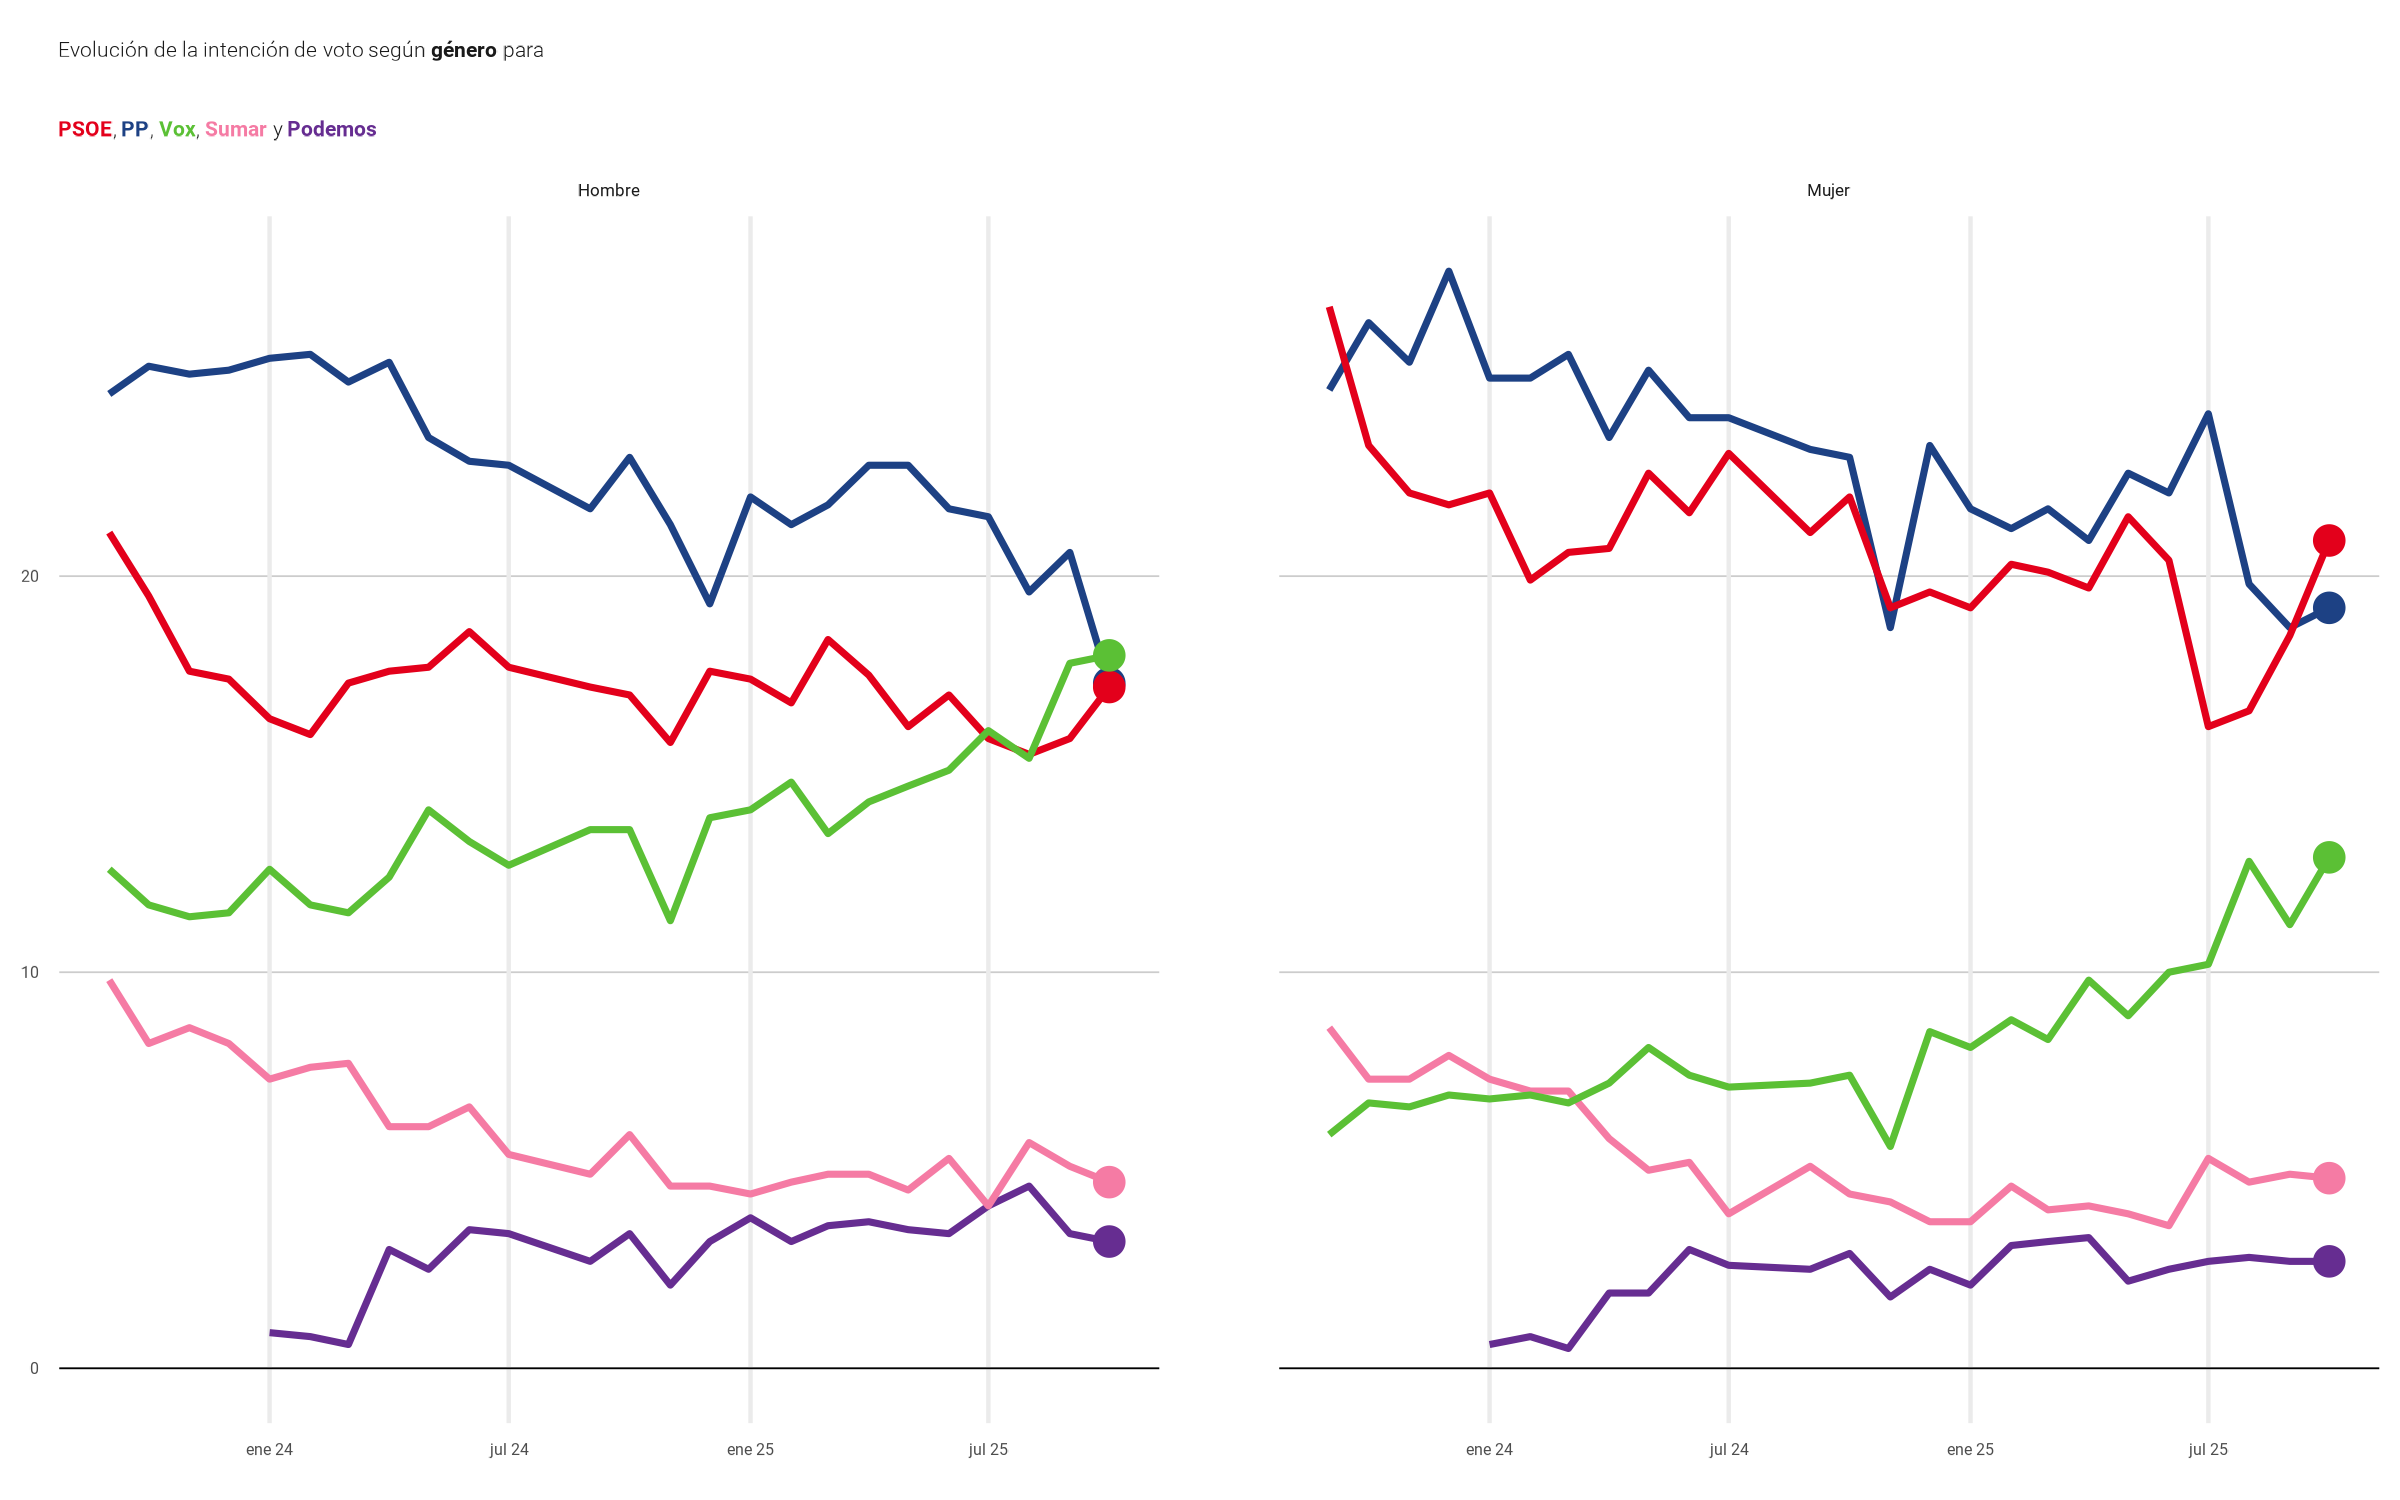
\includegraphics[width=8in,height=\textheight,keepaspectratio]{figures/p_idv_genero_static.png}




\end{document}
